\section{Approach}
In this section, we introduce \textbf{HaluAgent}, our proposed autonomous agent for detecting hallucinations across various text types. The core of our HaluAgent framework is a well-instructed LLM, which can autonomously leverage tools to detect a broader range of hallucination types. First, we define several tasks for hallucination detection and then design a toolbox with supporting tools to extend the LLM's capability. To enable step-by-step detection, we design a three-stage detection framework equipped with memory mechanism. Finally, we synthesize high-quality detection trajectory data to fine-tune open-source LLMs. We present the overall architecture of HaluAgent in Figure~\ref{fig: detection_framework}.


\begin{figure*}[tb]
	\centering
	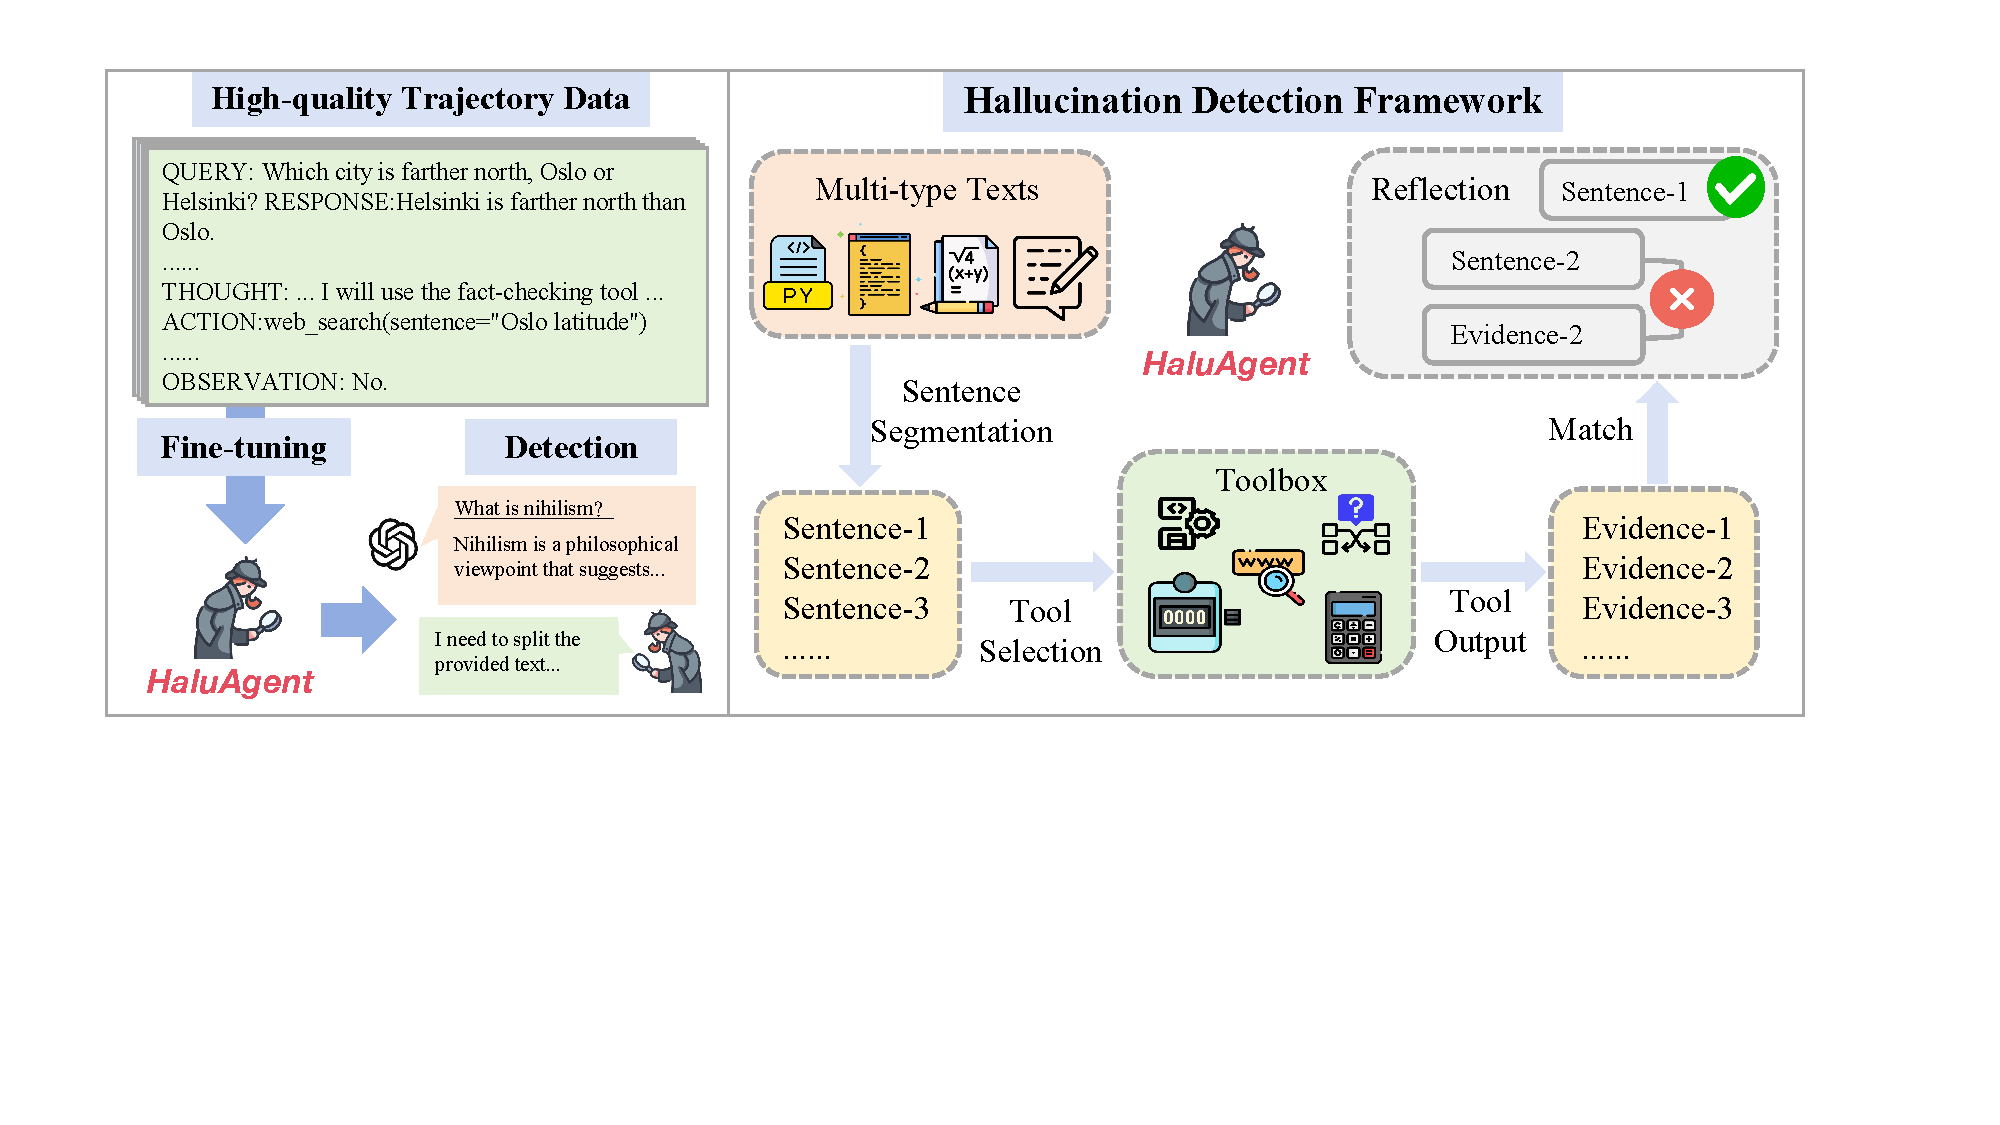
\includegraphics[width=1.00\textwidth]{image/HaluAgent.pdf}
	\caption{The overview of our proposed HaluAgent. The left part shows the process of fine-tuning open-source models and detecting hallucinations. The right part illustrates the hallucination detection pipeline of HaluAgent.}
	\label{fig: detection_framework}
	\vspace{-0.2cm}
\end{figure*}

\subsection{Task Definition}
\label{sec: task}
Hallucination refers to seemingly plausible yet factually unsupported content~\cite{huang2023survey}. Unlike previous work that mostly focused on detecting text-based hallucinations~\cite{manakul2023selfcheckgpt,InterrogateLLM}, we consider a broader range of hallucination forms such as text, code, and mathematical expression.
Hence, in this work, we conduct hallucination detection in five tasks as:

\textbullet~\textbf{Knowledge-based QA} involves generating answers to the input question~\cite{kbqa}, and we aim to identify misinformation from the answer text such as incorrect historical dates, misattributed quotes, or false scientific facts.

\textbullet~\textbf{Conditional Text Generation} focuses on tasks with specific requirements given in the input instructions~\cite{pplm} such as generating text with particular length, format, or translating 
a paragraph into special language. We aim to detect hallucinations that deviate from the given instructions or include irrelevant information.

\textbullet~\textbf{Semantic Consistency} is not specific to any particular type of text or task. We define hallucination in semantic consistency as those irrelevant or self-contradictory content in the responses.

\textbullet~\textbf{Math Problem Solving} is related to generating a series of mathematical expressions to solve the math problem~\cite{hendrycks2021measuring}, while the expressions may contain computational errors, \eg arithmetic or calculation mistakes.

\textbullet~\textbf{Code Generation} aims to generate code snippets for the input query~\cite{chen2021evaluating}. We define hallucinations as code snippets that are syntactically incorrect, fail to execute as intended, or contain logical flaws and missing dependencies.

Note that in real-world scenarios the responses from LLMs may contain a mixture of these hallucination types, and we aim to develop a general and versatile hallucination detection agent that can deal with a broader range of hallucinations.



\subsection{Toolbox for Hallucination Detection}
Since detecting texts with a mix of hallucination types is challenging, we design a comprehensive toolbox to enhance the hallucination detection capability of LLMs following previous work~\cite{chern2023factool,gou2024critic}. Based on the hallucination types discussed in Section~\ref{sec: task}, we incorporate five types of external tools, \ie search engine, calculator, code interpreter, condition verifier, and semantic checker, and two internal system tools: 

\textbullet~\textbf{Search Engine} is utilized to retrieve supporting evidence from the web for identifying factually incorrect content, defined as \emph{web\_search}.
We use Google Programmable Search Engine API\footnote{https://developers.google.com/custom-search} to implement this tool.
Considering the relevance between retrieved documents and the output text, we only use the top-5 documents as the most relevant retrieval results for hallucination detection.

\textbullet~\textbf{Calculator} is used to verify inaccurate mathematical calculations in the model responses, targeting math-related hallucinations, defined as \emph{calculator}.
We implement calculator via the scientific computing library SymPy~\cite{10.7717/peerj-cs.103}.

\textbullet~\textbf{Code Interpreter} can be used to validate code snippets by executing the snippets in a programming environment, defined as \emph{code\_interpreter}, ensuring that the code is syntactically correct and functions as intended. 
We implement the code interpreter tool following CRITIC~\cite{gou2024critic}.

\textbullet~\textbf{Condition Verifier} aims to detect hallucinations for conditional text generation by assessing whether the text is consistent with the given condition. For example, we utilize word counter (\emph{word\_counter}) to compute the number of words in a length-constrained generation scenario. 


\textbullet~\textbf{Semantic Checker} mainly addresses hallucination types such as irrelevant responses and self-contradictions, which is defined as \emph{match}. 
We leverage GPT-4 to examine the consistency and relevance of semantics, primarily handling the semantic matching scenario. 

\textbullet~\textbf{System Tools} are developed to support the basic manipulation operations for hallucination detection, including sentence segmentation (\emph{split\_text}) and returning detection results (\emph{get\_answer}).

All tools are defined as functions in a unified way and we present the whole toolbox in Table~\ref{tab: toolkit} in Appendix~\ref{app: toolkit}. It is worth noting that the toolbox is not limited to the existing tools and can be easily extended, \eg adding more task-specific tools.


\subsection{HaluAgent Framework}
\label{haluagent framework}

Inspired by prior work on complex reasoning~\cite{KGAgent}, we consider the hallucination detection process as an agent task. 
Specifically, HaluAgent includes three stages: sentence segmentation, tool selection, and reflection, along with memory mechanism. Below, we outline the workflow and components of our HaluAgent framework.

\paratitle{Sentence Segmentation.}
Since the responses of LLMs are usually the combination of facts, opinions, and various types of texts, we first segment the responses into several independent detection units. To be specific, we utilize the system tool, \textit{split\_text}, to perform sentence segmentation. This tool requires the agent to split the input text into a set of sentences and complete any incomplete semantic information within the sentences, \eg pronouns and omitted content.
Sentence segmentation reduces the complexity of hallucination detection tasks and allows HaluAgent to tailor its detection strategies for individual sentences, ensuring more accurate and fine-grained results by minimizing interference from unrelated content.


\paratitle{Tool Selection and Verification.}
Next, HaluAgent verifies each sentence separately by selecting the appropriate tool from the toolbox based on the type of sentence content (\eg \textit{web\_search} for fact statements and \textit{calculator} for mathematical expressions). HaluAgent compares each sentence with the execution results of the selected tool to identify any inconsistencies or inaccuracies, thereby detecting hallucinations.
To prevent the agent from forgetting intermediate detection results and support the subsequent reflection, HaluAgent stores the detection result of each sentence as a triple, \ie \emph{(sentence, hallucination label, supporting evidence)}. If the sentence is identified as containing hallucinations, it will be labeled ``1'', otherwise ``0''. These useful information will be stored based on a memory mechanism,
allowing HaluAgent to refer to historical results and maintain a consistent understanding of the text veracity throughout the detection process.

\paratitle{Reflection.}
After individually examining all the sentences, HaluAgent can obtain preliminary detection results. However, due to the limited capacity of each tool and potential errors in their outputs, these detection results might not be fully accurate. 
To address this, HaluAgent performs the final reflection to double-check whether the previous detection results are correct from \emph{local} and \emph{global} perspectives. At the local level, HaluAgent will match each sentence with the corresponding evidence to ensure the local correctness of hallucination detection. However, different sentences may influence each other. Therefore, at the global level, HaluAgent will determine whether the current sentence is incorrect based on the context of other sentences.
For instance, if the calculation result in a preceding sentence is incorrect, any subsequent steps based on this result should be considered incorrect, even if these steps are correct when checked in isolation.
Any detection mistakes will be corrected and the detection results (\ie hallucination label and supporting evidence) stored in memory are updated accordingly.
After reflection, HaluAgent invokes a system tool, \textit{get\_answer}, to output the final detection result. If any hallucinations are detected, HaluAgent outputs the specific sentences and supporting evidence from the detection tools.



Throughout the above process, HaluAgent first segments the input text into a set of semantically complete sentences, then selects tools to check each sentence individually, and finally reflects on the detection results to further correct mistakes. To support this process, we use memory mechanism to store useful information such as historical detection trajectories and current detection results.



\subsection{Bilingual Agent Tuning}

Previous studies mostly depended on closed-source LLMs (\eg GPT-4) to detect hallucinations~\cite{chern2023factool,wei2024long}. To empower smaller language models as effective hallucination detectors, we aim to perform supervised fine-tuning on smaller LLMs (\eg Baichuan2-Chat 7B). Given the powerful agent capability, we leverage GPT-4 to synthesize high-quality hallucination detection trajectory data in Chinese and English following the detection framework in Section~\ref{haluagent framework}. 


\subsubsection{Trajectory Generation}



\begin{table}[tb]
\centering
\small
\begin{tabular}{l|ccc}
\toprule
Datasets  & \#Train & \#Trajectory & \#Test \\
\midrule
WebQA & 900 & 675 & 100 \\
Ape210K & 500 & 334 & 100 \\
HumanEval & 100 & 100 & 63 \\
WordCnt & 100 & 100 & 100 \\
% \midrule
HaluEval-QA & 900 & 808 & 100 \\
\midrule
All & 2500 & 2017 & 463 \\
\bottomrule
\end{tabular}
\caption{Statistics of synthetic detection trajectories.}
\vspace{-0.3cm}
\label{tab: trajectory statistics}
\end{table}



\paratitle{Data Source.}
\label{sec: in-domain dataset}
To curate high-quality trajectory data covering diverse hallucination types, we select and construct five datasets, \ie HaluEval~\cite{li2023halueval} and WebQA~\cite{li2016dataset} for knowledge-based QA, Ape210K~\cite{zhao2020ape210k} for math word problem, HumanEval~\cite{chen2021evaluating} for code generation, and WordCnt for conditional text generation. Among them, HaluEval and HumanEval are English datasets, and WebQA, Ape210K, and WordCnt are Chinese datasets, which enable bilingual detection capabilities of HaluAgent. In our experiments, we use GPT-4 to synthesize WordCnt which is targeted at generating text with a specified length. Besides, we obtain the ground-truth hallucination labels for WebQA and Ape210K by ChatGPT and human annotators.
We provide details of each dataset in Appendix~\ref{app: data_source}.




\paratitle{Trajectory Format.}
Based on our datasets, we employ GPT-4 to execute the detection process in Section~\ref{haluagent framework} and generate corresponding trajectory data following the ReAct format~\cite{yao2023react}. We begin by feeding the detection instruction and the text to be detected as input for GPT-4. At each turn, the agent receives an \emph{observation}, makes its plans and thoughts as \textit{thought}, and invokes corresponding tools through \textit{action}. The results from these tools are formulated as a new observation for the next turn. By iterating the above process, we can obtain a complete detection trajectory comprising the input instruction, detected text, intermediate steps (\ie observations, thoughts, actions), and the final detection result. To ensure the accuracy of the trajectories, we remove those samples that include wrong tool invocation, formatting errors, and inconsistency between the detection result and the ground-truth hallucination label. Finally, we produce 2,017 high-quality trajectories for supervised fine-tuning. We present an example in Figure~\ref{fig: case study} and the statistics of trajectory data in Table~\ref{tab: trajectory statistics}.


\subsubsection{Trajectory Tuning}
Based on the above formatted bilingual trajectory data, we perform supervised fine-tuning on Baichuan2-Chat 7B and 13B~\cite{yang2023baichuan}, which are much smaller than the backbone models in previous studies~\cite{chern2023factool,wei2024long}. 
Formally, the hallucination detection trajectory for each sample can be represented as $\langle o_0, t_1, a_1, o_1, t_2, a_2, \ldots, o_{n-1}, t_n, a_n, o_n \rangle$, where $o_i$, $t_i$, and $a_i$ denote the observation, {thought}, and {action} at the $i$-th turn, respectively. Specifically, $o_0$ denotes the initial observation consisting of the input instruction and detected text, and $o_n$ denotes the final detection result. At each turn, based on the historical trajectory $c_i = \langle o_0, t_1, a_1, \ldots, o_{i-1} \rangle$, the agent aims to generate thought $t_i$ and action $a_i$.
Therefore, during the trajectory fine-tuning process, we only compute the cross-entropy loss for $t_i$ and $a_i$ while masking $o_i$:
\begin{equation}
    \mathcal{L} = -\log \sum_{i=1}^{n} \text{Pr}(t_i,a_i|c_i).
\end{equation}



\subsection{Comparison to Previous Work}

To clarify the differences between HaluAgent and other hallucination detection methods, we aim to address the following two questions:

\textbullet~\textbf{What are the benefits of designing an autonomous hallucination detection agent?} Hallucination detection is fundamental to related research. Most previous work either relied on the internal knowledge of LLMs (might be limited)~\cite{LMvsLM} or performed coarse-grained detection process~\cite{manakul2023selfcheckgpt}. Designing an agent for hallucination detection offers a flexible alternative that can effectively extend the detection capability of LLMs through tool utilization.
Existing agent-based detection methods do not consider tool utilization or only employ limited tools such as search engine for hallucination detection in long texts~\cite{lei2023chain,wei2024long}.
In contrast, HaluAgent develops a comprehensive and extensible toolbox and performs fine-grained reasoning process for hallucination detection, providing a more adaptable and robust solution.


\textbullet~\textbf{Can smaller language models perform well in challenging hallucination detection?}
Existing methods~\cite{chern2023factool, manakul2023selfcheckgpt, dhuliawala2023chain} heavily depended on powerful closed-source LLMs such as GPT-4, which leads to high computational costs and poses unavoidable limitations for the practical deployment of these technologies. Moreover, relying on closed-source models makes the detection results difficult to reproduce. 
Our work demonstrates that by incorporating the agent capabilities and tool integration, smaller language models can also effectively handle challenging hallucination detection tasks.
This way can provide a more viable and economical choice, significantly reducing the need for closed-source LLMs.


